\documentclass[12pt, notitlepage, final]{article} 

\newcommand{\name}{Vince Coghlan}

%\usepackage[dvips]{graphics,color}
\usepackage{amsfonts}
\usepackage{amssymb}
\usepackage{amsmath}
\usepackage{latexsym}
\usepackage{enumerate}
\usepackage{amsthm}
\usepackage{nccmath}
\usepackage{setspace}
\usepackage[pdftex]{graphicx}
\usepackage{epstopdf}
\usepackage[siunitx]{circuitikz}
\usepackage{tikz}
\usepackage{float}
\usepackage{cancel} 
\usepackage{setspace}
\usepackage{overpic}
\usepackage{mathtools}
\usepackage{listings}
\usepackage{color}
\usepackage{qtree}
%\usepackage{gensymb}

\usetikzlibrary{calc}
\usetikzlibrary{matrix}
\usetikzlibrary{positioning}

\numberwithin{equation}{section}
\DeclareRobustCommand{\beginProtected}[1]{\begin{#1}}
\DeclareRobustCommand{\endProtected}[1]{\end{#1}}
\newcommand{\dbr}[1]{d_{\mbox{#1BR}}}
\newtheorem{lemma}{Lemma}
\newtheorem*{corollary}{Corollary}
\newtheorem{theorem}{Theorem}
\newtheorem{proposition}{Proposition}
\theoremstyle{definition}
\newtheorem{define}{Definition}
\newcommand{\column}[2]{
\left( \begin{array}{ccc}
#1 \\
#2
\end{array} \right)}

\newdimen\digitwidth
\settowidth\digitwidth{0}
\def~{\hspace{\digitwidth}}

\setlength{\parskip}{1pc}
\setlength{\parindent}{0pt}
\setlength{\topmargin}{-3pc}
\setlength{\textheight}{9.0in}
\setlength{\oddsidemargin}{0pc}
\setlength{\evensidemargin}{0pc}
\setlength{\textwidth}{6.5in}
\newcommand{\answer}[1]{\newpage\noindent\framebox{\vbox{{\bf ECEN 5018 Spring 2014} 
\hfill {\bf \name} \vspace{-1cm}
\begin{center}{Homework \#5}\end{center} } }\bigskip }

\DeclareMathOperator*{\argmin}{arg\,min}

%absolute value code
\DeclarePairedDelimiter\abs{\lvert}{\rvert}%
\DeclarePairedDelimiter\norm{\lVert}{\rVert}
\makeatletter
\let\oldabs\abs
\def\abs{\@ifstar{\oldabs}{\oldabs*}}
%
\let\oldnorm\norm
\def\norm{\@ifstar{\oldnorm}{\oldnorm*}}
\makeatother

\def\dbar{{\mathchar'26\mkern-12mu d}}
\def \Frac{\displaystyle\frac}
\def \Sum{\displaystyle\sum}
\def \Int{\displaystyle\int}
\def \Prod{\displaystyle\prod}
%\def \P[x]{\Frac{\partial}{\partial x}}
%\def \D[x]{\Frac{d}{dx}}
\newcommand{\PD}[2]{\frac{\partial#1}{\partial#2}}
\newcommand{\PF}[1]{\frac{\partial}{\partial#1}}
\newcommand{\DD}[2]{\frac{d#1}{d#2}}
\newcommand{\DF}[1]{\frac{d}{d#1}}
\newcommand{\fix}[2]{\left(#1\right)_#2}
\newcommand{\ket}[1]{|#1\rangle}
\newcommand{\bra}[1]{\langle#1|}
\newcommand{\braket}[2]{\langle #1 | #2 \rangle}
\newcommand{\bopk}[3]{\langle #1 | #2 | #3 \rangle}
\newcommand{\Choose}[2]{\displaystyle {#1 \choose #2}}
\newcommand{\proj}[1]{\ket{#1}\bra{#1}}
\def\del{\vec{\nabla}}
\newcommand{\avg}[1]{\langle#1\rangle}
\newcommand{\piecewise}[4]{\left\{\beginProtected{array}{rl}#1&:#2\\#3&:#4\endProtected{array}\right.}
\newcommand{\systeme}[2]{\left\{\beginProtected{array}{rl}#1\\#2\endProtected{array}\right.}
\def \KE{K\!E}
\def\Godel{G$\ddot{\mbox{o}}$del}

%\onehalfspacing

\begin{document}

\answer{}

\textbf{1)} Consider the following cost sharing problem:
\begin{itemize}
  \item{Player set: $N=\{1,2,3\}$}
  \item{Opportunity costs: $c:2^N \rightarrow R$}
\end{itemize}
\[
  c(\{1\})=9\text{,  }\hspace{3mm}c(\{2\})=8\text{,  }\hspace{3mm}c(\{3\})=9
\]
\[
  c(\{1,2\})=14\text{,  }c(\{1,3\})=15\text{,  }c(\{2,3\})=13
\]
\[
  c(\{1,2,3\})=20\hspace{3cm}c(\{\emptyset\})=0\hspace{1cm}
\]

\begin{enumerate}[(a)]
  \item{Identify the core graphically}\\
    \begin{figure}[H]
    \begin{center}
    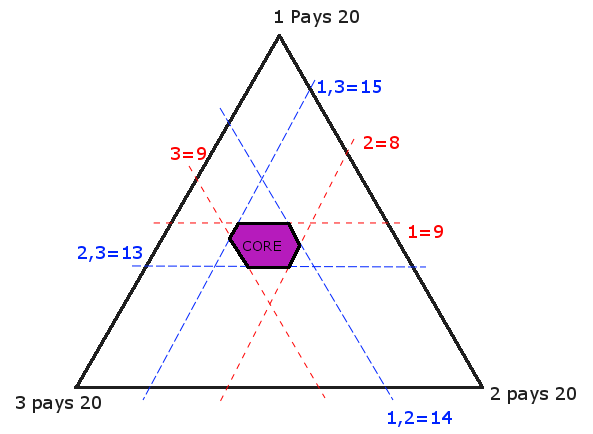
\includegraphics[width=9cm]{f1}
    \end{center}
    \end{figure}
  \item{Is the core nonempty?}\\
    Yes, as can be seen in the picture.
  \item{Compute the marginal contribution for each player.}\\
    The marginal cost of each player will be the marginal cost to the full coalition, for
    player 1:
    \[
      c(\{1,2,3\})-c(\{2,3\}) = 7
    \]
    for player 2:
    \[
      c(\{1,2,3\})-c(\{1,3\}) = 5
    \]
    and player 3:
    \[
      c(\{1,2,3\})-c(\{1,2\}) = 6
    \]
  \item{Compute the Shapley value for each player using equation in notes}\\
    The equation in the notes is:
    \[
      Sh(i,S;c)=\sum_{T\subseteq S\backslash\{i\}} \frac{|T|!(|S|-|T|-1)!}{|S|!}(c(T\cup\{i\})-c(T))
    \]
    For player 1:
    \[
      Sh(1,\{1,2,3\};c)=\frac{2}{6}(c(\{1,2,3\})-c(\{2,3\})) + \frac{1}{6}(c(\{1,2\})-c(\{2\})) + 
    \]
    \[
      \frac{1}{6}(c(\{1,3\})-c(\{3\})) + \frac{2}{6}(c(\{1\})-c(\{\emptyset\})) = 7\frac{1}{3}
    \]
    For player 2:
    \[
      Sh(2,\{1,2,3\};c)=\frac{2}{6}(c(\{1,2,3\})-c(\{1,3\})) + \frac{1}{6}(c(\{1,2\})-c(\{1\})) + 
    \]
    \[
      \frac{1}{6}(c(\{2,3\})-c(\{3\})) + \frac{2}{6}(c(\{2\})-c(\{\emptyset\})) = 5\frac{5}{6}
    \]
    For player 3:
    \[
      Sh(3,\{1,2,3\};c)=\frac{2}{6}(c(\{1,2,3\})-c(\{1,2\})) + \frac{1}{6}(c(\{1,3\})-c(\{1\})) + 
    \]
    \[
      \frac{1}{6}(c(\{2,3\})-c(\{2\})) + \frac{2}{6}(c(\{3\})-c(\{\emptyset\})) = 6\frac{5}{6}
    \]
  \item{Compute the Shapley value for each player using ordering approach in notes}\\
    The marginal contribution over all oderings can be easily calculated from the marginal
    values.  These must be found for each ordering, as seen below:
    \[
      3\leftarrow2\leftarrow1 \Rightarrow c(\{1,2,3\}) - c(\{2,3\}) = 7
    \]
    \[
      2\leftarrow3\leftarrow1 \Rightarrow c(\{1,2,3\}) - c(\{2,3\}) = 7
    \]
    \[
      2\leftarrow1\leftarrow3 \Rightarrow c(\{1,2\}) - c(\{2\}) = 6
    \]
    \[
      3\leftarrow1\leftarrow2 \Rightarrow c(\{1,3\}) - c(\{3\}) = 6
    \]
    \[
      1\leftarrow3\leftarrow2 \Rightarrow c(\{1\}) - c(\{\emptyset\}) = 9
    \]
    \[
      1\leftarrow2\leftarrow3 \Rightarrow c(\{1\}) - c(\{\emptyset\}) = 9
    \]
    For player 2:
    \[
      3\leftarrow1\leftarrow2 \Rightarrow c(\{1,2,3\}) - c(\{1,3\}) = 5
    \]
    \[
      1\leftarrow3\leftarrow2 \Rightarrow c(\{1,2,3\}) - c(\{1,3\}) = 5
    \]
    \[
      3\leftarrow2\leftarrow1 \Rightarrow c(\{2,3\}) - c(\{3\}) = 4
    \]
    \[
      1\leftarrow2\leftarrow3 \Rightarrow c(\{1,2\}) - c(\{1\}) = 5
    \]
    \[
      2\leftarrow3\leftarrow1 \Rightarrow c(\{2\}) - c(\{\emptyset\}) = 8
    \]
    \[
      2\leftarrow1\leftarrow3 \Rightarrow c(\{2\}) - c(\{\emptyset\}) = 8
    \]
    For player 3:
    \[
      2\leftarrow1\leftarrow3 \Rightarrow c(\{1,2,3\}) - c(\{1,2\}) = 6
    \]
    \[
      1\leftarrow2\leftarrow3 \Rightarrow c(\{1,2,3\}) - c(\{1,2\}) = 6
    \]
    \[
      2\leftarrow3\leftarrow1 \Rightarrow c(\{2,3\}) - c(\{2\}) = 5
    \]
    \[
      1\leftarrow3\leftarrow2 \Rightarrow c(\{1,3\}) - c(\{1\}) = 6
    \]
    \[
      3\leftarrow2\leftarrow1 \Rightarrow c(\{3\}) - c(\{\emptyset\}) = 9
    \]
    \[
      3\leftarrow1\leftarrow2 \Rightarrow c(\{3\}) - c(\{\emptyset\}) = 9
    \]
    We can then calculate the shapley value for each player, for player 1:
    \[
      \frac{1}{6}(7+7+6+6+9+9) = 7\frac{1}{3}
    \]
    for player 2:
    \[
      \frac{1}{6}(5+5+4+5+8+8) = 5\frac{5}{6}
    \]
    for player 3:
    \[
      \frac{1}{6}(6+6+5+6+9+9) = 6\frac{5}{6}
    \]
    Note that when we add these together we get 20.
  \item{Verify approaches in (d) and (e) result in the same answer.}\\
    Yes it is.
\end{enumerate}


\textbf{2)} Consider the following social choice problem with externalities:
\begin{itemize}
  \item{Three bidders $\{x,y,z\}$}
  \item{Three possible allocations $\{X,Y,Z\}$ where $X$ indicates object givin $x$}
  \item{Player specific valuations of allocations:}
    \begin{center}
      \begin{tabular}{c | c | c | c |}
        \multicolumn{4}{c}{\hspace{4mm} $X$ \hspace{2.7mm} $Y$ \hspace{2.7mm} $Z$}\\
        \cline{2-4}
        $x$ & 30 & 0 & -15 \\
        \cline{2-4}
        $y$ & 10 & 40 & 0 \\
        \cline{2-4}
        $z$ & 0 & -10 & 50 \\
        \cline{2-4}
      \end{tabular}
    \end{center}
\end{itemize}
\begin{enumerate}[(a)]
  \item{Discuss the VCG mechanism for this problem.  What allocation is chosen? What prices are charged
    to the players} \\
    The VCG mechanism will make an attempt to make the action of reporting your true value, the dominant
    strategy for any player.  We can see in this particular problem that $x$ would like to win the least,
    but also would like $z$ to lose the most.  $y$ would like to win the second most, but also wants $x$
    to win.  $z$ would like to win the most, but also wants $y$ to lose.  These externalities relate to
    the real life externalities that make designing mechanisms for games so hard.  We will see that the
    VCG mechanism will solve many of our problems.  The VCG mechanism is going to modify each player's
    bit as follows:
    \[
      \hat{b_x} = b_x+10 = 40
    \]
    \[
      \hat{b_y} = b_y-10 = 30
    \]
    \[
      \hat{b_z} = b_z-15 = 35
    \]
    And since $\hat{b_x}$ is the largest, player $x$ wins.  Both player $y$ and $z$ will pay nothing.
    player $x$ will now pay the second highest losing bid, minus 10.  He pays 25.

  \item{Prove that the VCG mechanism is efficient for this problem.} \\
    To prove that this is efficient we must prove two things, first that the game induces the players
    to report truthfully, and second, to provide the utilitarian social choice.  We will start with the
    first one.  Does player $y$ have any reason to bid anything other than his true value.  Let us see.
    Recall that the payoff for any player is:
    \[
      v_i(x^*(\hat{v}_i,\hat{v}_{-i})) + \sum_{j\neq i}\hat{v}_j(x^*(\hat{v}_i,\hat{v}_{-i})) - \sum_{j\neq i}\hat{v}_j(x^*(\hat{v}_{-i}))
    \]
    The desire to maximise this function means the desire of $y$ to maximise:
    \[
      v_y(x^*(\hat{v}_y,\hat{v}_{-y})) + \sum_{j\neq i}\hat{v}_j(x^*(\hat{v}_y,\hat{v}_{-y}))
    \]
    The amount he values a particular outcome added to the amount that everyone else values that
    outcome.  Player $y$ has the ability to pick any outcome he wants by altering his reported values. This
    is the nature of the VCG mechanism, $y$ has the ability to make any outcome occur.  $y$ wants to pick
    the outcome to maximize his own utility, by announcing his true value, he can assure that
    $x^*(v_y,\hat{v}_y)$ is the outcome that occurs.  This outcome maximizes $y$'s utility because if
    he were to value something different and still win, it wouldnt matter, since $\hat{v}_y$ is nowhere
    to be found in his utility function.  This is due to the fact that his final payment will be based
    only on the valuations of other players, of which he doesnt know.  If he were to lie and still lose,
    then either he would have won if he bid his true value, a case where his utility is negative, or
    he would have lost if he bid his true value, which makes no difference to him.  The only safe bet is
    to report the true value, anything else would be foolish.

    The utilitarian alternatice is:
    \[
      x^* \in \underset{x\in X}{\text{arg}\max} \sum_{i}v_i(x)
    \]
    in this case this set would look like $\{40,30,35\}$.  Note how this is exactly the change in bid that
    the VCG mechanism forces.  VCG is utilitarian by design.

\end{enumerate}

\textbf{3)}
\begin{enumerate}[(a)]
\item{Construct a two-player game that meets the following specifications:}
\begin{itemize}
  \item{The better reply graph has a cycle (i.e., it does \textit{not} have the finite inprovement property)}
  \item{The row player has 2 actions and the column player has 3 actions.}
  \item{There are no payoff "ties", i.e. a player is never indifferent between two actions.}
  \item{There is a unique pure Nash equilibrium.}
  Be sure to sketch the better reply graph.
\end{itemize}
To begin I will consider the following game:

\begin{center}
  \begin{tabular}{r |c|c|c|}
    \multicolumn{1}{r}{}
    & \multicolumn{1}{c}{L}
    & \multicolumn{1}{c}{C}
    & \multicolumn{1}{c}{R}\\
    \cline{2-4}
    T & 2,1 & 1,2 & 0,0\\
    \cline{2-4}
    B & 1,2 & 2,1 & 1,4\\
    \cline{2-4}
  \end{tabular}
\end{center}

Note that this satisfies the first qualification.  The cycle would look like:
$\{T,L\} \rightarrow \{T,C\} \rightarrow \{B,C\} \rightarrow \{B,L\}$.  Note that
this is for the better reply, not the best reply.  This cycle would not occur in
a system where the best reply was chosen, and in fact, no game of this size would
satisfy that.  Only a $3\times 3$ game would.  The second condition is clearly
satisfied.  The third condition is as well.  Each player has different values for
each action played by the other.  $\{B,R\}$ is also a unique pure Nash equilibrium.
It can be seen that at this point both players would not want to deviate. The better
reply graph would illustrate the cycle:

\begin{figure}[H]
\begin{center}
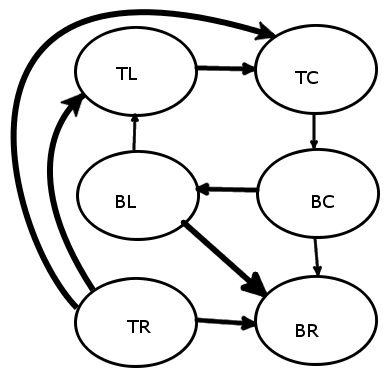
\includegraphics[width=8cm]{f2}
\end{center}
\end{figure}

\item{Is this possible when each player only has two moves?}\\
  No, in order to have a cycle in your graph, you must have a cycle of at least 4.  This is due to two facts:
  since two players can not make a unilateral change, a cycle must be an even number.  It cannot be two since
  that would mean that one player moves, then changes his mind, and moves back, but the payoff by definition
  would have to be different.  If your cycle has all four elements in it, then there can be no Nash equilibrium,
  since at each point, one player would want to move.
\end{enumerate}

\textbf{4)} Complete the payoffs in the following game so that it is a potential game:

\begin{center}
  \begin{tabular}{r |c|c|c|}
    \multicolumn{1}{r}{}
    & \multicolumn{1}{c}{L}
    & \multicolumn{1}{c}{C}
    & \multicolumn{1}{c}{R}\\
    \cline{2-4}
    T & 1,? & 2,? & 1,?\\
    \cline{2-4}
    M & ?,4 & 5,3 & 2,?\\
    \cline{2-4}
    B & 1,? & 6,? & 7,?\\
    \cline{2-4}
  \end{tabular}
\end{center}

I will rewrite this as:
\begin{center}
  \begin{tabular}{r |c|c|c|}
    \multicolumn{1}{r}{}
    & \multicolumn{1}{c}{L}
    & \multicolumn{1}{c}{C}
    & \multicolumn{1}{c}{R}\\
    \cline{2-4}
    T & 1,$a$ & 2,$b$ & 1,$c$\\
    \cline{2-4}
    M & $d$,4 & 5,3 & 2,$e$\\
    \cline{2-4}
    B & 1,$f$ & 6,$g$ & 7,$h$\\
    \cline{2-4}
  \end{tabular}
\end{center}

We need there to be a function $\Phi$ that satisfies the following property:
\[
  U_i(a'_i,a_{-i})-U_i(a_i,a_{-i}) = \Phi(a'_i,a_{-i}) - \Phi(a_i,a_{-i})
\]
We can preform a similar method as in class, set the center box to have a $\Phi$ of 0
and then move on from there, the first few calculations cane be easily figured:
\begin{center}
  \begin{tabular}{r |c|c|c|}
    \multicolumn{1}{r}{}
    & \multicolumn{1}{c}{L}
    & \multicolumn{1}{c}{C}
    & \multicolumn{1}{c}{R}\\
    \cline{2-4}
    T & 1-d,a-b & 2-5 & 1-2,c-b\\
    \cline{2-4}
    M & 4-3 & 0 & e-3\\
    \cline{2-4}
    B & 1-d,f-g & 6-5 & 7-2,h-g\\
    \cline{2-4}
  \end{tabular}
\end{center}

To be a potential game these have to be equal, for example:
\begin{center}
  \begin{tabular}{r |c|c|c|}
    \multicolumn{1}{r}{}
    & \multicolumn{1}{c}{L}
    & \multicolumn{1}{c}{C}
    & \multicolumn{1}{c}{R}\\
    \cline{2-4}
    T & 1,2 & 2,2 & 1,1\\
    \cline{2-4}
    M & 1,4 & 5,3 & 2,1\\
    \cline{2-4}
    B & 1,6 & 6,6 & 7,1\\
    \cline{2-4}
  \end{tabular}
\end{center}
Since there is a $\Phi$ for this game, it is a potential game.  $\Phi$ would look
like:
\begin{center}
  \begin{tabular}{r |c|c|c|}
    \multicolumn{1}{r}{}
    & \multicolumn{1}{c}{L}
    & \multicolumn{1}{c}{C}
    & \multicolumn{1}{c}{R}\\
    \cline{2-4}
    T & 0 & -3 & -1\\
    \cline{2-4}
    M & -1 & 0 & -2\\
    \cline{2-4}
    B & 0 & 1 & 5\\
    \cline{2-4}
  \end{tabular}
\end{center}

\textbf{5)} Consider the following two player game:
\begin{center}
  \begin{tabular}{r |c|c|}
    \multicolumn{1}{r}{}
    & \multicolumn{1}{c}{$a_2$}
    & \multicolumn{1}{c}{$b_2$}\\
    \cline{2-3}
    $a_1$ & 5,2 & 0,4\\
    \cline{2-3}
    $b_1$ & 0,4 & 2,6\\
    \cline{2-3}
  \end{tabular}
\end{center}

\begin{enumerate}[(a)]
\item{Suppose the one shot game defined above is repeated each day $t=0$,1,2,... and each
player uses the learning algorithm Ficticious Play to select their respective action at
time $t$.  If the initial action is $a(0) = (b_1,a_2)$ \textit{\textbf{derive}} the
ensuing action trajectory $a(1),a(2),...,a(n)$ for any $n>\geq 1$.}

The column player's best response is always to play $b_2$,  And its learning algorithm
will reflect this.  Player 1 is going to see player 2 continuously play $b_2$, which will
look to him like: $\beta_1(1) = (.5,.5)$, $\beta_1(2) = (.33,.67)$  in this way $\beta_1$ will be
\[
  \beta_1 = (\frac{1}{n},1-\frac{1}{n})
\]
Player 1's best response to $\beta_1(n)$ is going to be the maximization of:
\[
  \frac{1}{n}(p\cdot5) + (1-\frac{1}{n})((1-p)\cdot2)
\]
We can easily see how this will play out for the first few iterations:
\[
  a(0)=(b_1,a_2)\text{, }a(1)=(a_1,b_2)\text{, }a(2)=(a_1,b_2)\text{, }a(3)=(a_1,b_2)\text{, }
\]
\[
  a(4)=(b_1,b_2)\text{, }a(5)=(b_1,b_2)\text{,...}a(n)=(b_1,a_2)
\]
Player 1 seems to wise up in 4 moves.
\item{A Nash equilibrium $a*$ is strict if for any player $i$ and any action $a_i\neq a_i^*$}
\[
  U_i(a_i^*,a_{-i}^*) > U_i(a_i,a_{-i}^*)
\]
Consider \textit{any} two player game with finite action sets $\mathcal{A}_1$ and $\mathcal{A}_2$
Suppose each player uses the Ficticious play strategy.  Prove or disprove the following statement
\begin{center}
  \textit{If $a(t)$ is a strict Nash equilibrium, then $a(\tau) = a(t)$ for all times $\tau\geq t$.}
\end{center}
Does your answer from part (a) suggest that this statement is True or False?

I will start by saying that part (a) most definitely suggests that this statement is true, once
we arrive at a nash equilibrium, Ficticious Play sees no reason to deviate from this path.  It
makes sense, but lets prove it.  If we take some amount of time to arrive at a Nash equilibrium,
then we know that each player will have a best response for $t+1$:
\[
  a_i(t+1) = B_i(\beta_{-i}(t) + \frac{1}{t+1}(v[a_{-i}(t)] - \beta_{-i}(t)))
\]
where $v$ is the empirical frequencies:
\[
  v(t) = \begin{pmatrix}
    ... & \beta_a(t) \\
    ... & \beta_b(t)
  \end{pmatrix}
\]
We can find the utility of the next move:
\[
  U_i(a_i(t+1)) = \beta_aU_i(a_i(t)) + (1-\beta_a)U_i(b_i(t))
\]
Since $U_i(a_i) > U_i(a_i')$, and $U_i(b_i) > U_i(b_i')$.  We know that their
sum multiplied by positive numbers must also hold this fact and thus:
\[
\beta_aU_i(a_i(t)) + (1-\beta_a)U_i(b_i(t)) > \beta_aU_i(a_i'(t)) + (1-\beta_a)U_i'(b_i(t))
\]
And therefore:
\[
  U_i(a_i(t+1)) > U_i(a_i'(t+1))
\]
The very definition of a nash equilibrium.  Proving it for $t+1$ proves it inductively for
all $\tau\geq t$.

(c) Consider the Ficticious Play strategy generalized for more than two players.  In this
strategy each player $i$ does the following
\begin{itemize}
  \item{\textbf{Bookkeeping:} Maintains the empirical frequency of each player's previous
    actions.  Let $q_j(t) \in \Delta(\mathcal{A}_j)$ represent the empirical frequency of
  player $j$'s action over the stages $k=0,1,...,t-1$.}
  \item{\textbf{Assumptions:} Each player assumes that at any time $t$ each player $j\neq i$
    selects an action \textit{independently} using the strategy $q_j(t)$.}
  \item{\textbf{Best Response:} Each player selects an action at time $t$ seeking to maximize
    his expected utility (where his expectation is over his beliefs about the actions of the
  other players)
  \[
    a_i(t) = BR_i(q_{-i}(t))
  \]}
  \item{\textbf{Repeat:}}
\end{itemize}
Consider the following three player game:
\begin{center}
  \begin{tabular}{r |c|c|}
    \multicolumn{1}{r}{}
    & \multicolumn{1}{c}{$a_2$}
    & \multicolumn{1}{c}{$b_2$}\\
    \cline{2-3}
    $a_1$ & 0 & 1\\
    \cline{2-3}
    $b_1$ & 1 & 0\\
    \cline{2-3}
  \end{tabular}
  \begin{tabular}{r |c|c|}
    \multicolumn{1}{r}{}
    & \multicolumn{1}{c}{$a_2$}
    & \multicolumn{1}{c}{$b_2$}\\
    \cline{2-3}
    $a_1$ & 1 & -1\\
    \cline{2-3}
    $b_1$ & $x$ & 1\\
    \cline{2-3}
  \end{tabular}\\
  \vspace{2mm}
  \hspace{.9cm}$a_3$\hspace{2.2cm}$b_3$
\end{center}

This is a representation of a special type of game where the payoff of each player is the same,
i.e., for any action profile $a$, $U_i(a) = U_j(a)$ for any players $i$ and $j$.  Therefore, the
number in the payoff matrix represents the payoff to all players.  This type of game is called an
\textit{Identical Interest game}.

Suppose each player selects their action according to the prescribed fictitious play process.  Let
$a(0) = (a_1,a_2,a_3)$.
\begin{itemize}
  \item{Derive the ensuing action $a(1)$. Does $x$ have any impact?}\\
    The best response to $a(0)$ is $(b_1,b_2,b_3)$, so that is the next action, $x$ does not
    have an impact.
  \item{What is the expected utility for each player and each action at time 2?}\\
    At time 2, the empirical actions of the players are $(0.5,0.5,0.5)$.  And each player
    will best respond to that. This is where $x$ comes in.  If the probabilities are $p,q,r$ then
    the expected payoff for player 1 will be:
    \[
      p(q(r(0) + (1-r(1)))+(1-q)(r(1) + (1-r(-1)))) +
    \]
    \[
      (1-p)(q(r(1) + (1-r(x)))+(1-q)(r(0) + (1-r(1))))
    \]
    This means that player 1 will have to maximize:
    \[
      0.25(px+p-x+4)
    \]
    This is maximized when $x>-1$ by $p=1$ and when $x<-1$ it is $p=0$. For player 2 we can do a
    similar process:
    \[
      q(p(r(0) + (1-r(1)))+(1-p)(r(1) + (1-r(x)))) +
    \]
    \[
      (1-q)(p(r(1) + (1-r(-1)))+(1-p)(r(0) + (1-r(1))))
    \]
    This means that player 2 will have to maximize:
    \[
      0.25(5-qx-q)
    \]
    which is maximized when $x>-1$ by $q=0$ and when $x<-1$ it is $q=1$. Similarily for
    player 3:
    \[
      r(p(q(0) + (1-q(1)))+(1-p)(q(1) + (1-q(0)))) +
    \]
    \[
      (1-r)(p(q(1) + (1-q(-1)))+(1-p)(q(x) + (1-q(1))))
    \]
    Player 3 will want to maximize:
    \[
      0.25(5+x-r-rx)
    \]
    which is maximized when $x>-1$ by $r=1$ and when $x<-1$ it is $r=0$.  The new ficticious
    play best reply would be:
    \begin{displaymath}
   f(x) = \left\{
     \begin{array}{lr}
       (1,0,1) & x>-1\\
       (0,1,0) & x<-1\\
       ([0,1],[0,1],[0,1]) & x = -1
     \end{array}
   \right.
\end{displaymath} 

  \item{Consider \textit{any} game with $n>2$ players and finite action sets $\mathcal{A}_i$.
    Suppose each player uses the fictitious play strategy.  Prove or disprove teh following statement:}
\end{itemize}
\begin{center}
  \textit{If $a(t)$ is a strict Nash equilibrium, then $a(\tau) = a(t)$ for all times $\tau\geq t$.}
\end{center}
Does the presented three player game provide any insights?

The presented three player game provides an important insight into how we want to approach
this problem.  The Utility of the next move is going to be a very complicated expression.
Instead of a utility based off of the empirical probabilities of one person, they are
now based on multiple people.  For example, three players would make a payoff of:
\[
  U_i(a_i(t+1)) = \beta_c(\beta_bU_i(a_i(t)) + (1-\beta_b)U_i(b_i(t))) + (1-\beta_c)(\beta_bU_i(a_i(t)) + (1-\beta_b)U_i(b_i(t)))
\]
Note, however, that the proof is almost identical.  At any amount of players, the payoff
will be proportional to the utility of the last turn, and if the utility of the last turn
was a Nash equilibium, then we know that:
\[
  U_i(a_i(t)) > U_i(a_i'(t))
\]
and since they are proportional then,
\[
  U_i(a_i(t+1)) > U_i(a_i'(t+1))
\]
This is not supposed to be a vigourous mathematical proof since it was already done above
for the last problem.

\end{enumerate}


\end{document}
